%%
% The BIThesis Template for Graduate Thesis
%
% Copyright 2020-2023 Yang Yating, BITNP
%
% This work may be distributed and/or modified under the
% conditions of the LaTeX Project Public License, either version 1.3
% of this license or (at your option) any later version.
% The latest version of this license is in
%   https://www.latex-project.org/lppl.txt
% and version 1.3 or later is part of all distributions of LaTeX
% version 2005/12/01 or later.
%
% This work has the LPPL maintenance status `maintained'.
%
% The Current Maintainer of this work is Feng Kaiyu.
%
% Compile with: xelatex -> biber -> xelatex -> xelatex

\chapter{相关技术与工作}
\section{ELF文件结构}
ELF(Executable and Linkable Format)文件格式是目前类 Unix 操作系统(如 Linux、FreeBSD)中广泛采用的一种标准二进制格式,用于描述可执行文件、目标文件、共享库和内核转储文件。由于其良好的可扩展性与跨平台支持,ELF 格式被认为是现代操作系统中程序执行与链接的核心桥梁。一个典型的 ELF 文件主要包括以下四个关键结构:
\begin{enumerate} [label=\arabic*)] 
\item ELF 头(ELF Header)

ELF 文件的开头是一个固定大小的 ELF 头部,用于描述整个文件的总体信息。它包含了魔数(magic number)用于识别 ELF 文件、目标机器架构(如 x86、ARM)、文件类型(可执行文件、共享对象或目标文件)、程序入口地址、程序头表偏移、节头表偏移、各个表的数量与大小等。操作系统的加载器首先读取这一部分信息来判断该文件是否为合法的 ELF 文件,并根据提供的偏移值进一步解析程序头和节头信息。

\item 程序头表(Program Header Table)

程序头表是面向操作系统加载器的结构,主要描述程序运行时需要载入内存的“段”(Segment)。每一项描述了一个段的类型、在文件中的偏移、在内存中的虚拟地址、所需的权限(可读、可写、可执行)以及其大小等信息。例如,常见的代码段 .text、数据段 .data 等,都会在程序头表中有对应的段描述。加载器正是依据程序头表将相应部分映射至进程的地址空间中。

\item 节(Section)

节是编译和链接阶段使用的逻辑组织单元,用于存储源代码生成的不同类型的数据,如 .text(代码段)、.data(已初始化的数据段)、.bss(未初始化的数据段)、.rodata(只读数据)、.symtab(符号表)、.strtab(字符串表)、.debug(调试信息)等。节通常不会被直接加载进内存执行,而是由链接器使用,或被分析工具读取以进行二进制分析、反汇编和静态分析等任务。

\item 节头表(Section Header Table)

节头表则是面向链接器和调试器的结构,它记录了每个节的元信息,如名称、类型、权限、文件偏移、地址、大小等。每一项对应一个节,操作系统或工具链通过节头表来快速定位和解析各节内容。在某些可执行文件中,节头表甚至可以被省略,以减小文件体积或增加反分析难度,但这不会影响程序的加载运行,因为程序的执行依赖的是程序头表,而非节信息。

\end{enumerate}

\begin{figure}[hbt]
	\centering
	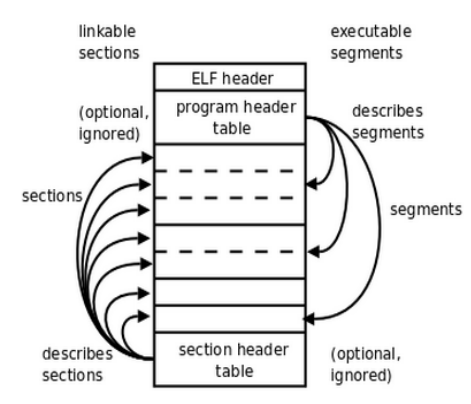
\includegraphics[width=0.75\textwidth]{figures/2.1}
	% \caption[这里的文字将会显示在 listoffigure 中]{这里的文字将会显示在正文中}
	\caption{ELF文件结构}\label{fig:2.1}
\end{figure}

\section{恶意软件检测技术}

随着信息技术的快速发展和应用系统的日益复杂,恶意软件在网络空间中的传播形式不断演化,攻击手段愈加隐蔽与智能化,传统的防护机制正面临严峻挑战。据全球网络安全厂商统计,2023年全球每天新增恶意软件样本超过50万个,其中近30\%的样本采用了变种、加壳、动态加载等手段以逃避检测,呈现出高度自动化和持续化的攻击特征。这些趋势表明,恶意软件检测正成为保障网络空间安全的关键技术环节。
目前,恶意软件检测技术主要分为以下三类,如图\ref{fig:2.2}所示:

\begin{figure}[hbt]
	\centering
	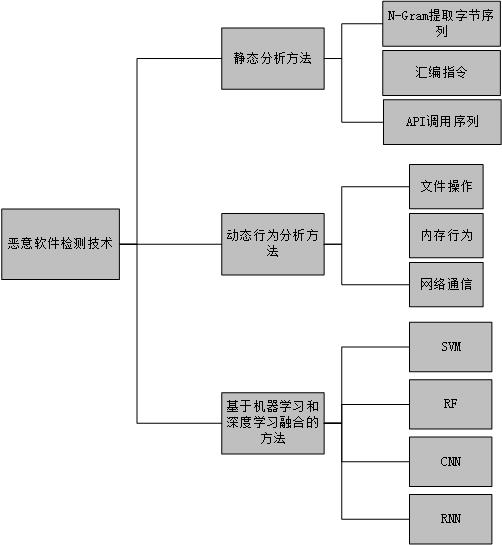
\includegraphics[width=0.75\textwidth]{figures/2.2}
	% \caption[这里的文字将会显示在 listoffigure 中]{这里的文字将会显示在正文中}
	\caption{恶意软件检测方法分类}\label{fig:2.2}
\end{figure}

%\begin{enumerate} [label=(\arabic*)] 

(1)静态分析方法

静态分析是最早应用于恶意代码检测的技术手段,主要通过对软件的二进制文件进行逆向工程分析,从中提取诸如特征码、字符串信息、导入表、节区结构、指令序列、操作码频率等静态特征,再使用签名匹配或机器学习方法进行分类判断。Kumar等\cite{kumar2019learning}通过组合PE头的原始值与派生值,并比较集成特征集与原始特征集,证明了基于前者的分类器能以较高准确度和较低成本检测和分类恶意软件。Yan等\cite{yan2019classifying}提出了一种利用深度图卷积神经网络对控制流图(CFG)进行嵌入的新型恶意软件分类系统,并在两个包含超过20,000个样本的大型数据集上验证了该系统的有效性。Corlatescu等\cite{corlatescu2023embersim}提出了基于静态分析的恶意软件检测框架,利用文件结构信息和元数据构建了EMBER基准数据集。Ling等\cite{ling2022malgraph}提出MalGraph,一种基于层次图神经网络的方法,用于鲁棒的Windows恶意软件检测,通过函数调用图和控制流图捕捉可执行文件的交互与结构语义。

该方法优点是速度快、资源消耗低,适合大规模样本初筛。但它的缺点也很明显:对经过加壳、混淆、代码插入等技术处理的恶意软件识别能力较弱,容易被绕过。

(2)动态行为分析方法

动态分析通过在虚拟沙箱或受控环境中执行可疑程序,监控其运行时的行为,包括系统调用序列、文件操作、注册表修改、网络通信等动态特征,以此判断程序的恶意性。Trizna等\cite{trizna2024nebula}提出了一种名为Nebula的自注意力Transformer架构,用于动态恶意软件分析。通过对行为报告进行标记化、过滤、归一化和编码,适配Transformer架构,并进行全面消融研究,评估系统组件对性能的影响。Bhat等\cite{bhat2023system}利用系统调用分析对Android应用进行动态行为分析,提取动态特征后,使用集成学习算法分类。Li等\cite{li2022novel}在安全虚拟环境中对软件API调用序列进行动态分析,并将这些序列转化为多种特征表示,使用深度学习模型(包括Bi-LSTM)进行分类。Chen等\cite{chen2022cruparamer}提出了基于参数增强的API序列学习方法,通过深度神经网络训练,具有较高的检测鲁棒性和泛化能力。Rohini等\cite{rohini2024magic}提出MAGIC方法,通过行为共现和回归分析量化恶意软件行为,实验结果显示MAGIC比传统方法更准确地反映签名的恶意程度,提高了恶意软件威胁的防御能力。

这种方法更侧重于检测实际行为,因此在应对变种或混淆样本方面具有更好的鲁棒性。然而,其缺点在于分析开销较大,容易被延时执行或沙箱检测绕过。此外,一些高度针对性的APT攻击样本在沙箱中可能不会暴露其真实行为,从而导致漏报。

(3)基于机器学习和深度学习融合的方法

近年来,随着人工智能技术的快速发展,越来越多的研究者将机器学习与深度学习方法应用于恶意软件检测任务。通过从样本中提取静态或动态特征,再使用如支持向量机(SVM)、随机森林(RF)、卷积神经网络(CNN)、循环神经网络(RNN)等模型进行分类训练,已在多个公开数据集上取得了较好的检测效果。Ngo等\cite{ngo2023fast}提出了一种结合静态和动态特征的快速恶意软件检测方法,利用迁移学习提升检测效率。通过深度学习提取潜在特征表示,解决特征维度不一致的问题,并使用知识蒸馏技术将聚合特征的知识迁移到静态特征模型中,实现快速检测。Shar等\cite{shar2023experimental}从Android应用中提取14种特征,比较传统机器学习(如随机森林)和深度学习(如循环神经网络)在这些特征上的表现。Bashir等\cite{bashir2024hybrid}提取Android应用的静态和动态特征(如API调用和权限),并使用SVM、K-NN、NB及集成学习方法分类。

恶意软件检测技术正从传统的签名匹配逐渐迈向智能化、自适应的发展方向。Bensaoud和Kalita\cite{bensaoud2022deep}通过生成恶意软件的位图和PNG图像并输入深度学习模型进行分类,采用硬参数共享和软参数共享策略,成功检测使用各种混淆技术的恶意软件。Conti等\cite{conti2022few}提出了一种基于GEM图像的深度学习方法,结合灰度矩阵图像、GLCM纹理特征、马尔可夫图像和熵图像,用于较浅的CNN架构,提升了训练和分类效率。Mallik等\cite{mallik2022conrec}通过将恶意软件样本转为灰度图像,并利用卷积神经网络捕捉结构相似性,结合BiLSTM层和VGG16层的输出,进行恶意软件家族分类,表现出色。

尽管检测方法不断优化,但随着攻击者技术手段的日益多样化,现有检测系统仍难以全面覆盖所有威胁类型,尤其是对抗性样本的出现,进一步揭示了现有模型的脆弱性。因此,如何在保证检测准确率的同时,提升模型对抗攻击的鲁棒性,成为当前恶意软件检测领域的重要研究方向之一。

该方法具有一定的自适应能力和特征抽象能力,但其检测结果往往依赖于训练数据的分布一致性,面对对抗样本或新型威胁时仍存在鲁棒性不足的问题。
%\end{enumerate}

\section{对抗性恶意软件}
近年来,随着深度学习技术在恶意软件检测中的广泛应用,基于神经网络的分类模型成为主流检测手段之一。然而,大量研究发现,深度神经网络虽然在标准测试样本上表现出色,却容易受到“对抗样本(Adversarial Examples)”的干扰。攻击者通过对输入数据添加轻微但精心设计的扰动,能够误导模型做出错误判断。这种攻击方式在图像识别、语音识别等领域已有广泛研究,并逐步扩展到网络安全领域,尤其是恶意软件检测。

所谓对抗性恶意软件(Adversarial Malware),是指攻击者在不破坏原有恶意功能的前提下,对恶意样本进行精细化扰动,使其在被检测时被误识为正常程序,从而绕过检测系统。这些扰动可以在代码层面(如指令插入、控制流调整)、结构层面(如节表改写、符号表扰动),或行为层面(如API调用序列伪装)实施,具有高度隐蔽性和针对性。


与图像等静态数据不同,恶意软件样本具有复杂的执行语义和潜在行为逻辑,因此对抗性样本的生成不仅要保证样本在结构上的有效性,更要保持其原始攻击行为的可执行性。这一特点使得恶意软件领域的对抗样本生成问题更加复杂与挑战性更高。


目前已有多种方法被提出用于生成对抗性恶意软件,主要包括以下几类:


基于梯度的扰动方法:如FGSM\cite{lupart2023study}(Fast Gradient Sign Method)、PGD\cite{bryniarski2021evading}(Projected Gradient Descent)等方法,将样本视为向量,通过计算模型梯度找到最易引发误判的方向添加扰动。但此类方法大多适用于图像等连续空间,对可执行文件中的离散结构处理效果有限。


启发式与搜索方法:这类方法将扰动操作建模为搜索问题,利用遗传算法\cite{wang2022black}、模拟退火\cite{bertsimas1993simulated}、蒙特卡洛树搜索\cite{chaslot2010monte}等手段,在可执行性约束下寻找最佳扰动路径。其优点是可定制性强,但搜索效率与样本质量之间常常存在权衡。

基于强化学习的方法:近年来,强化学习(RL)因其在策略学习方面的优势,逐渐成为对抗样本生成研究的热点。攻击者构建一个智能体,以规避检测系统为奖励目标,学习一系列扰动策略。常见方法如基于Q-learning\cite{watkins1992q}、DQN\cite{osband2016deep}、PPO\cite{yu2022surprising}(Proximal Policy Optimization)等。这类方法能在保证样本合法性的前提下,实现自适应扰动策略的学习与优化。

对抗性恶意软件的研究不仅揭示了现有检测系统的潜在脆弱性,也推动了鲁棒性检测模型和对抗训练机制的快速发展。然而,如何在扰动成本、逃逸能力和语义一致性之间取得平衡,仍是该领域面临的核心挑战之一。尤其是在对抗样本跨模型迁移性、抗演化检测能力方面,仍需深入研究。

\section{强化学习}

强化学习(Reinforcement Learning, RL)是一种基于试错机制(trial and error)进行学习的人工智能方法,其核心思想是智能体(Agent)通过与环(Environment)的交互,在获得奖励信号的基础上不断调整策略,以最大化长期收益。与监督学习不同,强化学习并不依赖于明确的标签信息,而是通过环境反馈学习行为的价值,具有较强的自适应性与在线学习能力,因而广泛应用于博弈策略优化、机器人控制、自然语言处理及对抗样本生成等任务中。

强化学习过程通常可以使用马尔可夫决策过程(Markov Decision Process, MDP)建模,MDP由一个五元组(S, A, P, R, γ)构成,其中表示所有可能的环境状态的集合。每一个状态刻画了当前环境的完整信息,它是Agent进行决策时观察到的依据。表示所有可能的动作或行为的集合。Agent在某一特定状态下可以选择一个动作  来与环境进行交互。 定义了环境的动态变化规律,即在状态下采取动作后转移到下一个状态的概率,通常表示为:这一性质体现了马尔可夫性,即下一个状态只与当前状态和当前动作有关,与过去的历史无关。 是即时奖励函数,表示在状态  下采取动作后,环境给予Agent的即时反馈,记为 。奖励信号用于指导Agent的学习过程,使其调整行为以获取更多的累计奖励。 是一个折扣因子,用于平衡短期奖励与长期奖励的重要性。较小的  倾向于让Agent更关注近期的奖励,而较大的则鼓励Agent考虑长期累积收益。

\begin{figure}[hbt]
	\centering
	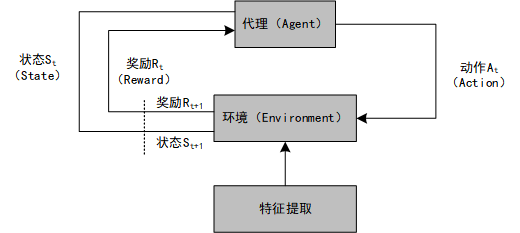
\includegraphics[width=0.75\textwidth]{figures/2.3}
	% \caption[这里的文字将会显示在 listoffigure 中]{这里的文字将会显示在正文中}
	\caption{马尔可夫决策过程}\label{fig:2.3}
\end{figure}

在实际的强化学习交互过程中,智能体(Agent)遵循以下步骤循环进行:
\begin{enumerate} [label=\arabic*)] 
	
\item 观察状态:在时间步 ,Agent观察到当前的环境状态 。
\item 选择动作:基于当前策略 ,Agent选择一个动作 。
\item 执行动作并反馈:动作  作用于环境,环境根据转移概率  跳转到下一个状态 ,并反馈一个即时奖励 。
\item 更新策略(学习):Agent利用所得到的状态、动作、奖励以及新的状态信息更新其内部策略,以期在未来做出更优的决策。

\end{enumerate}

强化学习的目标是学习一个最优策略 ,使得在任意状态下采取的动作能够最大化未来的累计奖励。累计奖励定义为从当前时刻  开始,未来各时刻奖励的折扣和:
\begin{equation}
	\label{eq:reward}
	\boldsymbol{G}_t = \sum_{k=0}^{\infty} \gamma^k r_{t+k}
\end{equation}

其中,\( r_{t+k} \) 表示从时刻 \( t \) 开始第 \( k \) 步时获得的奖励;\( \gamma^k \) 表示第 \( k \) 步奖励的折扣因子。

在强化学习中,策略(Policy)是指导智能体在不同状态下选择动作的规则。策略可以是确定性的,也可以是随机性的。策略优化是强化学习的核心目标之一,常见的方法包括直接优化策略的梯度方法,如策略梯度(Policy Gradient)算法\cite{silver2014deterministic},以及近些年提出的PPO\cite{yu2022surprising}(Proximal Policy Optimization)、TRPO\cite{schulman2015trust}(Trust Region Policy Optimization)等更稳定、高效的优化方法。策略优化关注的是如何基于交互经验调整智能体的行为,以更好地达成目标。

除了直接优化策略之外,强化学习中还广泛使用价值函数(Value Function)来间接指导策略改进。价值函数评估智能体在特定状态或状态-动作对上能够获得的期望累计奖励,通常包括状态价值函数V(s)和动作价值函数Q(s,a)。通过对价值函数的学习,智能体能够更有针对性地选择动作。价值函数的估计可以通过动态规划(如价值迭代、策略迭代)、蒙特卡洛方法\cite{chaslot2010monte}(Monte Carlo Methods)、或时间差分学习\cite{tesauro1991practical}(Temporal Difference Learning)等技术来实现。

强化学习过程中,智能体面临探索(Exploration)与利用(Exploitation)的权衡问题。探索意味着尝试新的、未验证过的动作,以期发现更优的决策路径;而利用则是依据已有知识选择当前认为最优的动作以获取最大回报。如何在探索和利用之间达到合理平衡,直接影响学习效率和最终性能。常见的探索机制包括ε-贪婪策略\cite{wunder2010classes}(Epsilon-Greedy)、基于置信上界\cite{auer2002finite}(Upper Confidence Bound, UCB)的方法、以及基于策略熵的鼓励机制(Entropy Regularization)。

强化学习方法可以根据是否需要建模环境动态而划分为基于模型(Model-Based)和无模型(Model-Free)两大类。基于模型的方法试图学习环境的状态转移规律和奖励机制,从而通过模拟来提高学习效率,如Dyna-Q\cite{peng2018deep}算法。相比之下,无模型的方法则直接根据交互数据学习策略或价值函数,无需显式推断环境模型,代表算法包括深度Q网络(DQN)、策略梯度方法等。基于模型的方法在样本效率上具有潜在优势,但通常面临模型误差带来的累积偏差问题。

近年来,深度强化学习\cite{li2019deep}(Deep Reinforcement Learning, DRL)技术的兴起,使得强化学习能够处理高维、复杂的输入空间。通过引入深度神经网络作为策略函数或价值函数的近似器,DRL极大地拓展了强化学习的应用边界。例如,DQN使用卷积神经网络处理原始像素输入,成功在Atari游戏中达到人类水平;而DDPG、A3C、PPO等方法则将深度学习与连续控制任务结合,在机器人控制、自动驾驶等领域表现出色。深度强化学习的挑战主要在于训练不稳定性和样本效率问题,因此在研究中引入了经验回放、目标网络、归一化技术等一系列改进措施。

此外,面对复杂任务和长时间尺度的决策需求,强化学习也发展出层次化学习(Hierarchical Reinforcement Learning, HRL)\cite{nachum2018data}的方法。通过引入子任务(Options)或多层次的策略结构,HRL能够在抽象层次上分解决策问题,提升学习效率和泛化能力。层次强化学习方法如FeUdal Networks、Options Framework在多阶段任务规划中展现了明显优势。

在多智能体环境中,强化学习技术进一步拓展到多智能体强化学习(Multi-Agent Reinforcement Learning, MARL)领域。MARL研究多个智能体在同一环境中相互作用、竞争或协作的学习过程。针对多智能体系统中策略非平稳性的问题,提出了集中式训练与分布式执行(CTDE)框架、对抗性自博弈(Self-Play)等方法,广泛应用于博弈决策、群体智能、对抗训练等方向。

总体来看,强化学习技术体系涵盖了从基础建模到复杂策略优化、从单智能体学习到多智能体协作的广泛内容。随着计算能力提升和算法不断创新,强化学习正在成为解决复杂智能决策问题不可或缺的重要技术。

\section{神经网络与时序建模技术}

神经网络(Neural Networks)是一类模拟人脑神经元结构与运行机制的计算模型,广泛应用于图像识别、自然语言处理、智能决策等领域。其基本结构包括输入层、一个或多个隐藏层和输出层。每一层通过权重连接前一层神经元,并使用激活函数引入非线性能力,使网络能够逼近任意复杂的非线性映射关系。

神经网络的核心优势在于其强大的表示能力,尤其在数据量充足的情况下,能够自动学习数据中的高阶抽象特征,替代传统人工设计特征的方式,大幅提升模型的泛化性能与适应能力。

在安全领域,神经网络已被用于恶意软件检测、异常行为识别、攻击流量检测等任务,并取得显著成果。然而,由于很多安全任务具有时间依赖性强、上下文联系紧密、行为逻辑复杂等特点,传统的前馈神经网络往往无法有效捕捉这些动态特征。

\subsection{循环神经网络(RNN)}

循环神经网络(Recurrent Neural Network,RNN)是一种专门用于处理序列数据的神经网络模型,其核心特点是具有“记忆能力”,即在处理当前输入时能够利用以往时间步的信息。与传统前馈神经网络不同,RNN的隐藏层神经元不仅接收当前时刻的输入,还接收上一个时刻隐藏层的输出,从而实现了对时间序列的依赖建模。这种结构使RNN特别适合处理语言文本、语音、视频帧序列等具有时间顺序的数据。

在RNN中,每一个时间步的计算会将上一个时间步的状态(隐藏层的输出)传递到下一个时间步,并结合当前输入进行处理,实现序列中信息的传递和积累。但在实际训练过程中,由于反向传播时梯度要经过多个时间步回传,RNN容易出现“梯度消失”或“梯度爆炸”的问题,导致模型在长序列中难以捕捉长期依赖关系。

\begin{figure}[hbt]
	\centering
	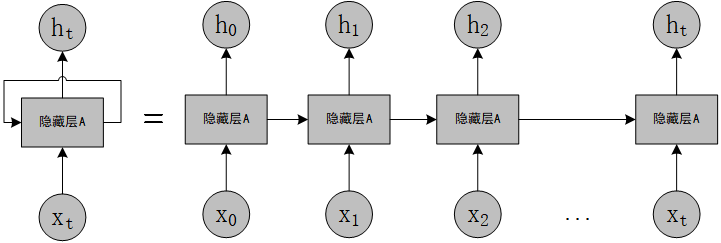
\includegraphics[width=0.75\textwidth]{figures/2.4}
	% \caption[这里的文字将会显示在 listoffigure 中]{这里的文字将会显示在正文中}
	\caption{RNN神经网络结构}\label{fig:2.4}
\end{figure}

为了解决这一问题,研究者提出了多种改进结构,其中最具代表性的是长短期记
忆网络(Long Short-Term Memory, LSTM)和门控循环单元(Gated Recurrent Unit, GRU)。这些改进模型通过引入门控机制(如输入门、遗忘门、输出门)来控制信息
的流入、保留和输出,有效缓解了传统 RNN 在长序列建模中的不足。

RNN及其变种在诸多序列建模任务中展现出强大的性能,特别是在自然语言处
理、机器翻译、语音识别、恶意行为序列建模等领域中,为强化学习、时序建模和序
列生成等应用提供了坚实的基础。

\subsection{长短期记忆网络(LSTM)}

长短期记忆网络(Long Short-Term Memory,LSTM)\cite{graves2012long}是一种特殊的循环神经网络(RNN)结构,旨在解决传统RNN在处理长序列数据时面临的“梯度消失”和“梯度爆炸”问题。与传统RNN相比,LSTM通过引入精心设计的“门控机制”,能够在序列中选择性地记住或忘记信息,从而有效捕捉长期依赖关系,广泛应用于自然语言处理、语音识别、时间序列预测等任务。

LSTM的核心结构包含三个门控单元:输入门(Input Gate)、遗忘门(Forget Gate)和输出门(Output Gate),以及一个单元状态(Cell State),用于携带长期记忆信息。

输入门:控制当前输入信息中哪些部分可以被写入到记忆单元中;

遗忘门:决定前一时刻的记忆状态中哪些信息应该被保留、哪些应该被遗忘;

输出门:则决定当前时刻的记忆状态中哪些内容将作为隐藏状态传递到下一时刻。

LSTM的关键是通过这三个门的配合,实现对信息流的精确控制,从而保留对模型预测有用的信息,丢弃无用或冗余的信息。其信息流如下:首先,遗忘门根据当前输入和前一时刻的隐藏状态,决定哪些旧信息要被“遗忘”;接着,输入门决定要将多少当前输入的新信息写入记忆单元;然后,更新记忆状态;最后,输出门根据当前记忆状态输出一个隐藏状态,用于传递到下一个时间步。
LSTM的这种设计使得它可以在长序列中持续保留有效信息,并忽略无关部分,克服了传统RNN在长距离依赖建模方面的劣势。

\begin{figure}[hbt]
	\centering
	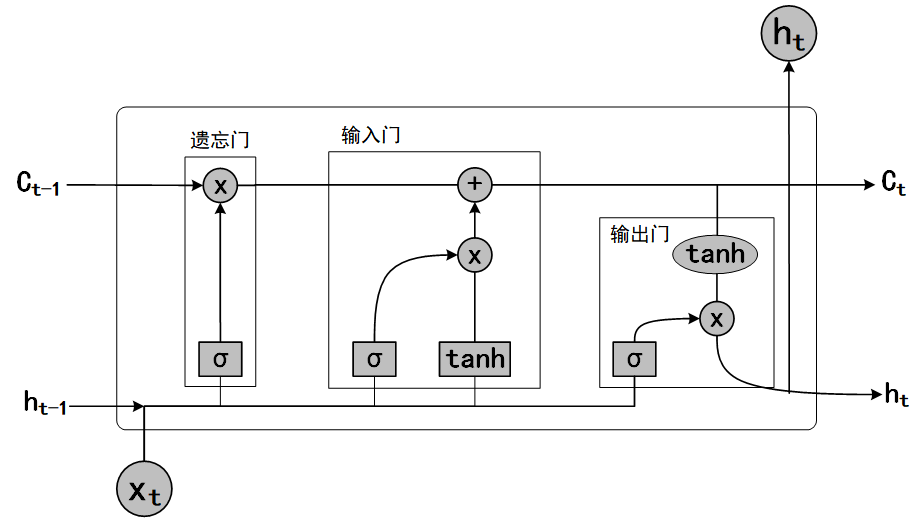
\includegraphics[width=0.75\textwidth]{figures/2.5}
	% \caption[这里的文字将会显示在 listoffigure 中]{这里的文字将会显示在正文中}
	\caption{LSTM基本数据单元结构}\label{fig:2.5}
\end{figure}

由于恶意软件的行为特征和扰动操作本质上具有明显的时序依赖性和上下文联系。恶意样本在执行过程中会形成一系列调用序列、系统行为或指令流,这些序列中的上下文信息对判断恶意行为及实施有效扰动具有重要价值。传统的全连接神经网络或标准循环神经网络(RNN)在处理这类时序数据时,往往难以保持长期依赖,容易遗忘序列中早期的关键信息。而 LSTM 网络通过引入门控机制(包括输入门、遗忘门和输出门),能够有效控制信息的记忆与遗忘,从而保留长期依赖关系,提升模型对扰动序列语义结构的建模能力。具体而言,在生成扰动策略时,LSTM 能够根据当前样本结构状态和历史扰动操作,动态调整策略输出,从而生成更具“攻击性”同时又具备高隐蔽性的对抗扰动。这种记忆能力对于生成具有“顺序逻辑”且能逃避检测系统的恶意行为非常关键。

\section{PPO}

Proximal Policy Optimization(PPO)\cite{yu2022surprising}是一种基于策略梯度的强化学习算法,由 OpenAI 于 2017 年提出。作为 Trust Region Policy Optimization(TRPO)的改进版本,PPO 保留了 TRPO 中稳定更新策略的核心思想,同时大幅简化了算法的实现和训练流程。由于其良好的稳定性与效率,PPO 已成为深度强化学习领域中应用最广泛、表现最为稳定的算法之一。

PPO 的核心思想在于限制新旧策略之间的变化幅度,从而避免策略在更新过程中发生剧烈波动,保证学习过程的稳定性。与传统策略梯度方法直接最大化目标不同,PPO 引入了裁剪目标函数(clipped objective)或基于 KL 散度的惩罚项,用以约束新旧策略的差异。

在裁剪目标函数形式下,PPO 的优化目标为:
\begin{equation}
	\boldsymbol{r}_t(\theta) = \frac{\boldsymbol{\pi}_\theta(\boldsymbol{a}_t | \boldsymbol{s}_t)}{\boldsymbol{\pi}_{\theta_{\text{old}}}(\boldsymbol{a}_t | \boldsymbol{s}_t)}
\end{equation}

其中,\( \boldsymbol{r}_t(\theta) \) 表示当前策略与旧策略在动作概率上的比值。通过最小化裁剪后的目标函数,可以有效防止策略更新偏离旧策略过远,从而提升训练过程的稳定性。

PPO具有诸多显著优势。其稳定性强,通过引入“剪切”目标函数限制每一步策略更新的幅度,从而有效避免了策略在训练过程中发生剧烈变化或崩溃的问题,提升了训练的可靠性。其次,PPO易于实现,相较于 TRPO(Trust Region Policy Optimization)等算法,不需要进行二阶导数计算或求解复杂的约束优化问题,因此更易于在工程中部署和调试,拥有更好的实用性。此外,PPO 还展现出良好的泛化能力,适用于多种不同类型的任务和环境,尤其在处理高维状态空间、复杂交互场景(如机器人控制、游戏智能体)中表现出色。其结构简单但高效,适配性强,可与卷积神经网络、循环神经网络等多种深度结构结合,有助于应对不同形式的输入数据(如图像、序列等)。

在本文所研究的对抗性恶意软件样本生成任务中,PPO 展现出独特的应用优势。由于扰动策略优化本质上是一个非线性且动态变化的过程,同时需要在保持样本功能完整性的前提下逐步施加扰动,PPO 通过平稳且高效的策略更新机制,为智能体提供了持续优化扰动策略的能力,避免了因剧烈策略变动而导致样本失效的问题。

因此,PPO 成为本文对抗性恶意软件扰动策略学习的核心算法之一。其稳定的策略优化特性与优异的泛化性能,为生成高效、隐蔽且具有迁移能力的对抗样本提供了坚实的技术保障。

\begin{figure}[hbt]
	\centering
	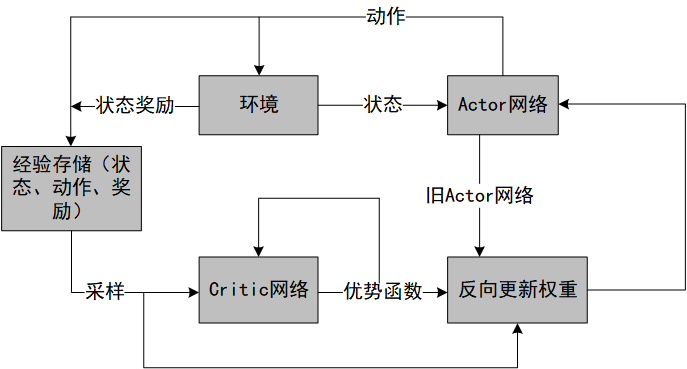
\includegraphics[width=0.75\textwidth]{figures/2.6}
	% \caption[这里的文字将会显示在 listoffigure 中]{这里的文字将会显示在正文中}
	\caption{PPO强化学习模型结构}\label{fig:2.6}
\end{figure}

\section{本章小结}

本章围绕ELF文件结构、恶意软件检测技术、对抗性恶意软件及强化学习四个方面展开了详细介绍。首先,从结构层面对ELF文件的基本组成进行了分析,重点阐述了ELF头、程序头表、节区及节头表在程序执行与加载过程中的作用。接着,介绍了当前主流的恶意软件检测技术,包括静态分析、动态行为分析以及基于机器学习和深度学习的方法,明确了各类方法的优劣和适用场景。在此基础上,进一步探讨了对抗性恶意软件的基本概念、生成方式及其对现有检测系统带来的挑战,指出对抗性样本具有极高的隐蔽性与攻击性,是当前研究中的热点难点问题。最后,本章简要回顾了强化学习的基本原理与流程,并结合恶意软件扰动任务,分析了其在对抗样本生成中的应用潜力。


